\begin{figure}[h]
  \centering
  \captionsetup{justification=centering}
  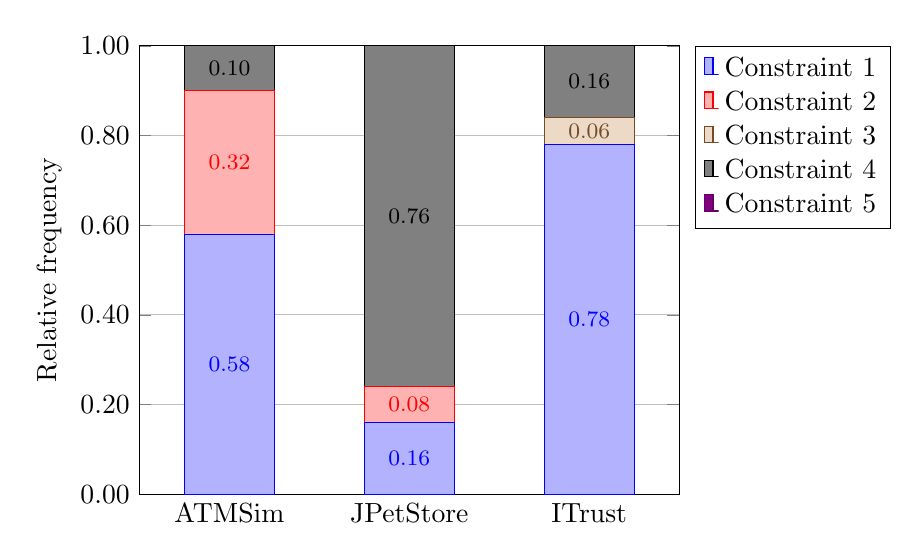
\begin{tikzpicture}\pgfkeys{
     /pgf/number format/precision=2, 
    /pgf/number format/fixed zerofill=true,
    /pgf/number format/fixed
}
  
    \begin{axis}[
        ybar stacked,
        ymajorgrids = true,
        nodes near coords,
        every node near coord/.append style={font=\footnotesize},
        xbar legend,
%         nodes near coords align={right},
        legend pos=outer north east,
        enlarge x limits=0.25,
        enlarge y limits=false,
        bar width=.5,
        % x axis
        xtick={1,2,3},
        xticklabels={ATMSim,JPetStore,ITrust},
        %x tick label style={rotate=45,anchor=east},
        % y axis
        ymin=0,
        ylabel={Relative frequency},
      ]
     % C1
     \addplot+[ybar] plot coordinates {(1,0.58) (2,0.16) 
      (3,0.78)};
     % C2
    \addplot+[ybar] plot coordinates {(1,0.32) (2,0.08) 
      (3,0)};
     % C3
    \addplot+[ybar] plot coordinates {(1,0) (2,0)
      (3,0.06)};
     % C4
    \addplot+[ybar] plot coordinates {(1,0.1) (2,0.76) 
      (3,0.16)};
     % C5
    \addplot+[ybar] plot coordinates {(1,0) (2,0) 
      (3,0)};
      

      \legend{Constraint 1,Constraint 2,Constraint 3, Constraint 4, Constraint 5}
    \end{axis}
  \end{tikzpicture}

  \caption{The relative frequency of constraint violations found in the three projects.}
  \label{bar:rel_frequency_violation_compraison}
\end{figure}